%
%-----------------------------------
\newpage
\section{Narrow Line Magneto-Optical Trap}
%-----------------------------------
%

\begin{wrapfigure}{l}{0.4\textwidth}
    \centering
    \vspace{-10px}
    \caption{Atomic cloud shape in nMOTs for small laser intensities.}
    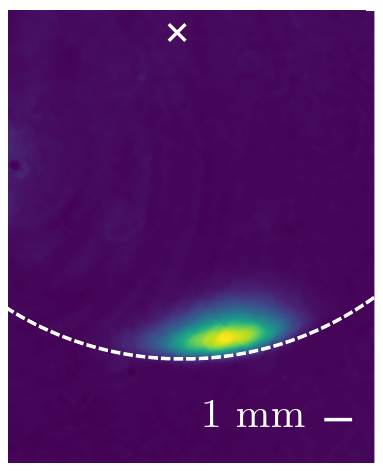
\includegraphics[width=0.3\textwidth]{USPSC-img/atomic_cloud_shape_in_nMOTs.png}
    \legend{Typical \textit{in situ} absorption image of an atomic sample in a nMOT. \\ Source: \cite{dreon2017optical}}
    \label{fig:atomic-cloud-shape-nMOTs}
    \vspace{-10px}
\end{wrapfigure}

In previous sections, we have been neglecting the gravity effect on the MOT parameters. This assumption is valid when the MOT force is much higher than gravity. The maximum radiation pressure force on an atom is $ \hbar k \Gamma / 2 $ from equation (\ref{eq:1D-MOT-force-components}). Therefore, the ratio between the maximum radiation pressure force and gravity is
\begin{equation}
    R \equiv \frac{\hbar k \Gamma}{2 m g},
    \label{eq:gravity-radiation-force-ratio}
\end{equation}
where $ m $ is the atomic mass and $ g $ is the gravitation acceleration. Usually, $ R $ is on the order of $ 10^5 $. Hence, the gravity force is negligible since the radiation pressure force is much higher. However, the lower $ \Gamma $, the higher the gravity effect so that for $ \Gamma \sim\ \textrm{kHz} $, the ratio (\ref{eq:gravity-radiation-force-ratio}) approaches values on the order of $ 10 $. In this case, the centre of mass moves towards the gravity direction such that, for small laser intensities, the atoms gather on the bottom of the surface of an ellipsoid as illustrated in figure \ref{fig:atomic-cloud-shape-nMOTs}.

Furthermore, $ \Gamma $ also defines the average number of scattering events per time (\textbf{scattering rate}) so that the lower $ \Gamma $, the fewer the number of events in a determined time interval. We have been analysing the atoms dynamics classically through the optical forces, which assumes that there are a large number of momentum exchange in a small period of time. In this condition, we can average out a force. That is not satisfied when $ \Gamma $ is sufficient smaller. In this case, we must include the discrete momentum exchange in the analysis and then treat the dynamics quantum mechanically. To quantify the range of $ \Gamma $ in which this happens, let us define the ratio given by
\begin{equation}
    \eta = \frac{\Gamma}{\omega_R}
    \label{eq:eta-ratio}
\end{equation}
where $ \hbar \omega_R $ is the kinetic energy $ (\hbar k)^2 / (2 m) $ gain by the atom when it absorbs an photon with the momentum $ \hbar k $. This energy is known as \textbf{photonic recoil}. When $ \eta \leq 1 $, one scattering event is able to detune the atom-light interaction. A MOT whose $ \eta \sim 1 $ or less is known as \textbf{narrow-line magneto-optical trap} (nMOT), whereas a MOT whose $ \eta \gg 1 $ is known as \textbf{broad-line magneto-optical trap}.


%-----------------------------------
\subsection{Operating regimes}
\label{sec:nMOT-operating-regimes}
%-----------------------------------

Four quantities play a crucial role in nMOTs operating: the saturation parameter $ s_0 $, the laser detuning $ \delta $, the natural linewidth $ \Gamma $, and the photonic recoil $ \omega_R $. We can combined $ s_0 $ and $ \Gamma $ in a single quantity known as \textbf{power-broadened linewidth} $ \Gamma' \equiv \Gamma \sqrt{1 + s_0} $, which is the natural energy scale of the atom-light interaction due to the power-broadening mechanism (section \ref{sec:line-broadening-mechanisms}). Furthermore, we can summarize those quantities in two essential quantities that characterized nMOTs:
\begin{itemize}
    \item ($ \eta' \equiv \Gamma' / \omega_R $): it defines the relevance of single scattering events to the the atom-light interaction taking the natural energy scale into account. Hence, $ \eta' $ is more accurate than $ \eta $;
    \item ($ \delta' \equiv \delta / \Gamma' $): it defines the coupling strength between atom and light normalized by the natural energy scale of the interaction.
\end{itemize}
When $ \eta' \gg 1 $, the semiclassical approach is suitable since the photonic recoil is much lower than the natural energy scale and, therefore, the scattering events can be averaged out. There are three nMOTs regimes:
\begin{enumerate}
    \item[I] \textbf{Doppler regime} ($ \eta' \gg 1 $ and $ |\delta'| < 1 $): in this regime, gravity is negligible so that the atomic cloud is ellipsoidal;
    \item[II] \textbf{Power-broadened regime} ($ \eta' \gg 1 $ and $ |\delta'| > 1 $): In this regime, gravity is comparable to the radiation pressure forces such that the atomic cloud centre of mass sags to vertical positions.
    \item[III] \textbf{Quantum regime} ($ \eta' \sim 1 $): in this regime, the photonic recoil is the natural energy scale and, therefore, the quantum physics governs the nMOT dynamics.
\end{enumerate}

%-----------------------------------
\subsection{Centre of mass of the atomic cloud}
\label{sec:nMOT-centre-of-mass}
%-----------------------------------

We can estimate the centre of mass of the atomic cloud in the power-broadened regime by assuming that all radiation pressure forces on an atom balance each other in all directions except in the gravity direction. In this case, the gravity force balances with the radiation pressure forces in the same direction. Let us consider red-detuned lasers such that $ \delta' < 0 $ and $ |\delta'| > 1 $. We expected that the centre of mass $ z_0 < 0 $, where the origin is the point at which the magnetic field is zero. Furthermore, we also expected that the the magnetic field component in the gravity direction will be much larger than the other components so that we can assume the magnetic field entirely in the gravity direction. In these conditions, the forces (\ref{eq:1D-MOT-force-components}) are valid in the gravity directions.
